\chapter{I Had to Beg, Borrow, and Steal: Capital, Control, and the Arithmetic of Scale}

This chapter follows a School of Hard Knocks interview with Louis, a Houston entrepreneur whose labor-force management company is described in the transcript as doing about \$300 million in annual revenue. The chapter is curated by LazyingArt LLC through Video2Book. There are no validated blackboard equations or diagrammatic screenshots for this lecture, so the mathematics below is deliberately modest: ratios, timing gaps, debt reduction, equity control, and results-based pricing reconstructed from the spoken record.

\section{The Opening Number}

The interview begins with spectacle: a Ferrari, a Houston street encounter, a private car collection, and the claim of a \$300 million company. But the first serious number is not the value of the cars. It is Louis's answer to a question about delegation.

He says the company will do about \$300 million in revenue this year, and that if he were still doing everything himself, it might do about \$3 million. Let
\[
R_{\mathrm{org}} \approx \$300\text{M/year},
\qquad
R_{\mathrm{solo}} \approx \$3\text{M/year}.
\]
The rough leverage of organization over personal labor is therefore
\begin{equation}
L_{\mathrm{delegation}}
   \approx
   \frac{R_{\mathrm{org}}}{R_{\mathrm{solo}}}
   \approx
   \frac{300}{3}
   =
   100.
\end{equation}

We should not read this as a formal proof that delegation alone caused a hundredfold increase. It is a scale contrast. The point is that the business has crossed from the work one owner can personally perform into work performed by a managed organization.

\subsection{Question \& Answer}

\paragraph{Question.} What did delegation multiply?

\paragraph{Answer.} It multiplied operating capacity. Louis's comparison is between a founder-centered firm and an organization that can act through people, procedures, authority, and management. The spoken arithmetic, \$300 million versus maybe \$3 million, gives us a rough 100x managerial leverage claim.

\section{What Was Being Built}

The next question restores the mechanism behind the display. Louis says FX is a labor-force management company: it partners with companies across the United States, and those companies outsource their entire labor force to it.

That is more precise than simply selling labor hours. In the transcript, the business object contains several pieces:
\begin{itemize}
\item a customer with a labor-force problem,
\item a provider that manages the labor system,
\item contracts large enough to require working capital,
\item operating procedures and training,
\item customer relationships that can expand over time.
\end{itemize}

\begin{definition}
A \emph{managed labor-force contract}, as used here, is an arrangement in which a customer transfers responsibility for a substantial labor function to an outside operator. The operator must staff, finance, manage, and improve the work before all customer cash has necessarily arrived.
\end{definition}

This definition matters because it prepares the capital problem. A small service job can sometimes be funded out of pocket. A large labor-force contract creates payroll and operating obligations before the invoice is collected.

\subsection{Question \& Answer}

\paragraph{Question.} What did Louis actually sell?

\paragraph{Answer.} From the transcript, he sold labor-force management. The customer was not merely buying individual workers; it was outsourcing an operating burden. That is why customer trust, payroll timing, SOPs, and financing all become part of the same story.

\section{Mindset, Risk, and Retained Earnings}

Before the interview reaches invoice factoring, it passes through mindset and spending. This sequence is easy to compress too aggressively, but it motivates the later financial discipline.

Louis says mindset matters more than skill set because skills can be taught, while passion, drive, and risk tolerance cannot simply be handed over. He also says entrepreneurship is not for everyone. The risk and mental strain can make the work unhealthy for some people.

Then the conversation turns to spending. The interviewer raises the claim that one in four millionaires live paycheck to paycheck; we keep that as an interview claim rather than an independently verified statistic. Louis's mechanism is still clear: high income does not protect someone who converts cash into consumption debt.

A compact way to write the warning is
\begin{equation}
\text{financial fragility rises when}
\quad
\text{consumption debt} >
\text{productive investment}.
\end{equation}

Louis then applies the same logic to the business. He says every dollar made each week had to stay in the company to reduce the next week's debt liabilities. Let \(D_t\) be the borrowing need at period \(t\), and let \(RE_t\) be retained earnings left inside the firm. The spoken rule is approximated by
\begin{equation}
D_{t+1} \approx D_t - RE_t.
\end{equation}
This is not a full accounting model. It is the discipline he describes: do not extract the cash, reduce the expensive borrowing, and build the balance sheet.

The next transition is natural. If growth is necessary, and growth consumes cash before it produces collected cash, then retained earnings become more than prudence. They become fuel.

\section{The Price of Seed Money}

The interviewer then asks the capital question directly. Many founders need money to start or grow. Louis answers by distinguishing two cases: funding an untested idea and funding proven scale.

If a founder has only an idea, the investor is carrying the financial downside. The founder risks time and sweat equity, but if the project fails, the investor loses the money. Therefore, Louis says, the investor wants control over how that money is spent. In equity language, that can mean majority control:
\begin{align}
s_{\mathrm{investor}} &\geq 51\%,\\
s_{\mathrm{investor}} &\approx 70\%,
\qquad
s_{\mathrm{founder}} \approx 30\%.
\end{align}

These are Louis's interview figures, not universal laws. They describe the bargain when one side supplies most of the financial risk before proof of execution.

\subsection{Question \& Answer}

\paragraph{Question.} Why does seed money cost so much ownership?

\paragraph{Answer.} Because control follows risk. If the investor funds a raw idea and bears the downside, the investor wants authority over spending and usually wants majority ownership. A founder with revenue, proof of concept, and evidence of execution is in a different position: the outside money is funding scale, not just possibility.

\begin{figure}
\centering
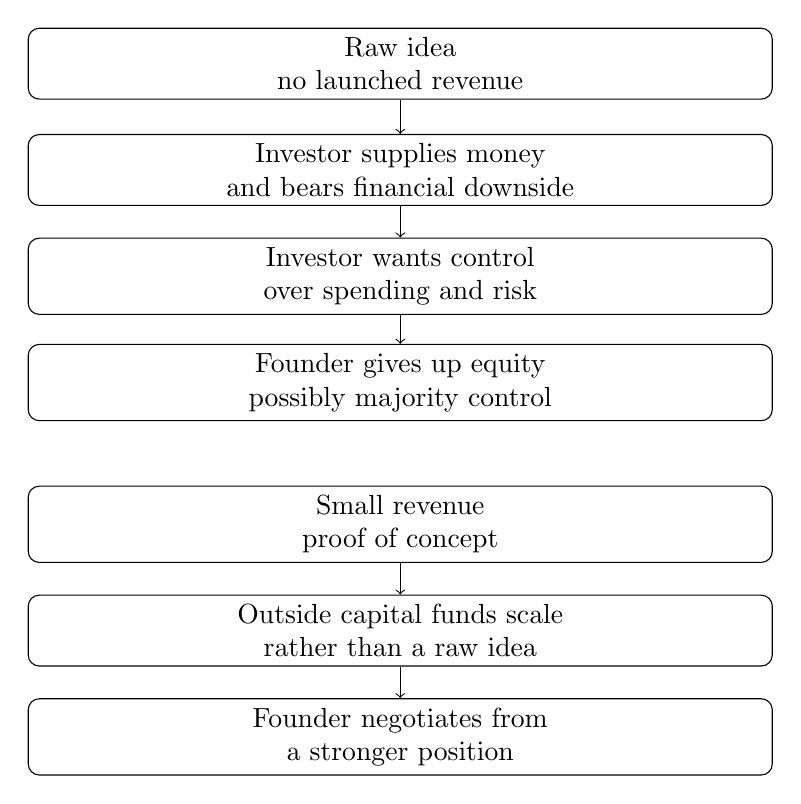
\begin{tikzpicture}[
  node/.style={draw, rounded corners, align=center, text width=0.76\linewidth, minimum height=0.9cm}
]
\node[node] (idea) at (0,0) {Raw idea\\no launched revenue};
\node[node] (risk) at (0,-1.35) {Investor supplies money\\and bears financial downside};
\node[node] (control) at (0,-2.70) {Investor wants control\\over spending and risk};
\node[node] (dilution) at (0,-4.05) {Founder gives up equity\\possibly majority control};

\node[node] (proof) at (0,-5.85) {Small revenue\\proof of concept};
\node[node] (scale) at (0,-7.20) {Outside capital funds scale\\rather than a raw idea};
\node[node] (position) at (0,-8.55) {Founder negotiates from\\a stronger position};

\draw[->] (idea) -- (risk);
\draw[->] (risk) -- (control);
\draw[->] (control) -- (dilution);
\draw[->] (proof) -- (scale);
\draw[->] (scale) -- (position);
\end{tikzpicture}
\caption{Transcript-derived capital path. Raw ideas tend to invite investor control; proof of concept improves the founder's bargaining position.}
\end{figure}

\section{The Working-Capital Gap}

Now the interview reaches its central arithmetic. Louis says his first major deal was about \$9 million a year, annualized. The customer needed 30-day payment terms. But expenses did not wait 30 days. He says that with the 30-day term plus a fifth week of expenses going out, the business had to cash-flow about five weeks and needed roughly \$1 million.

Let
\[
R_1 \approx \$9\text{M/year},
\qquad
T_{\mathrm{pay}} = 30\text{ days},
\qquad
N_{\mathrm{weeks}} \approx 5.
\]
If \(E_{\mathrm{week}}\) denotes weekly cash outflow, a cautious reconstruction is
\begin{equation}
B_{\mathrm{needed}} \approx E_{\mathrm{week}}N_{\mathrm{weeks}},
\end{equation}
with Louis's spoken estimate
\begin{equation}
B_{\mathrm{needed}} \approx \$1\text{M}.
\end{equation}

\subsection{A Scale Check}

We should not infer an exact payroll model. The transcript does not give gross margin, payroll timing, tax timing, or operating expenses. But the annualized revenue number gives a rough scale:
\begin{equation}
\frac{\$9\text{M}}{52}
\approx
\$173{,}000\text{ per week}.
\end{equation}
Five weeks at that revenue scale gives
\begin{equation}
5 \times \$173{,}000 \approx \$865{,}000,
\end{equation}
which is close to the spoken ``about a million'' estimate. This is only an order-of-magnitude check. It explains why a profitable contract can still be dangerous if the cash arrives late.

Louis used invoice factoring, or accounts receivable factoring. Each week he presented invoices; the factoring company advanced cash against them. He describes the advance as around 90 percent of invoice value and the all-in cost as about 21 percent:
\begin{align}
A_{\mathrm{cash}} &\approx 0.90I,\\
i_{\mathrm{factoring}} &\approx 21\%.
\end{align}
Here \(I\) is the invoice face value, \(A_{\mathrm{cash}}\) is the cash advance, and \(i_{\mathrm{factoring}}\) is the spoken all-in financing cost.

\begin{figure}
\centering
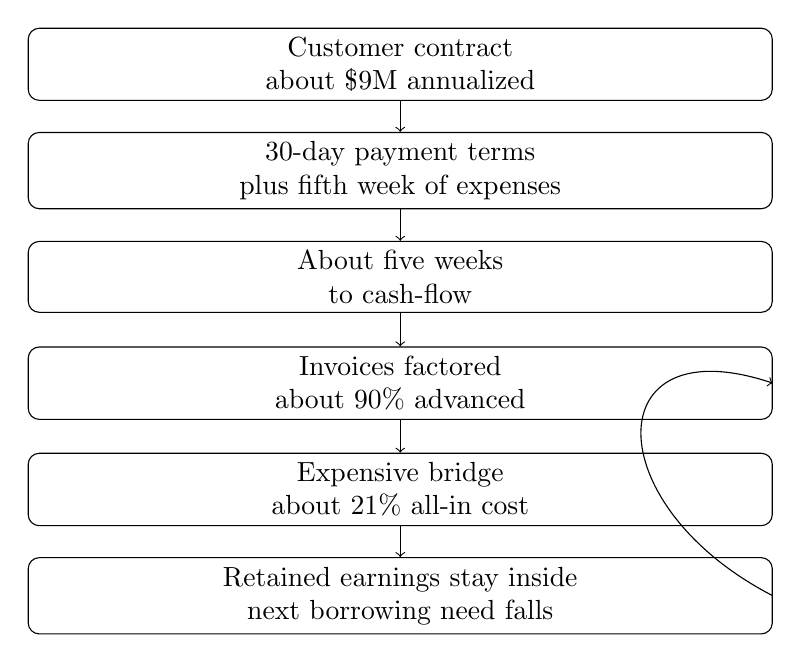
\begin{tikzpicture}[
  node/.style={draw, rounded corners, align=center, text width=0.76\linewidth, minimum height=0.9cm}
]
\node[node] (contract) at (0,0) {Customer contract\\about \$9M annualized};
\node[node] (terms) at (0,-1.35) {30-day payment terms\\plus fifth week of expenses};
\node[node] (gap) at (0,-2.70) {About five weeks\\to cash-flow};
\node[node] (factor) at (0,-4.05) {Invoices factored\\about 90\% advanced};
\node[node] (cost) at (0,-5.40) {Expensive bridge\\about 21\% all-in cost};
\node[node] (discipline) at (0,-6.75) {Retained earnings stay inside\\next borrowing need falls};

\draw[->] (contract) -- (terms);
\draw[->] (terms) -- (gap);
\draw[->] (gap) -- (factor);
\draw[->] (factor) -- (cost);
\draw[->] (cost) -- (discipline);
\draw[->] (discipline.east) .. controls (2.5,-5.6) and (2.5,-3.3) .. (factor.east);
\end{tikzpicture}
\caption{Transcript-derived working-capital bridge. Factoring supplies cash before collection, but retained earnings gradually reduce the need for expensive borrowing.}
\end{figure}

The narrative turn is important. Louis calls the factoring money horrible. He compares it to loan-shark money. But he also says it taught discipline: he could not pay himself for a long time, and each dollar left inside the company meant borrowing a little less the next week. Painful capital became an operating constraint that preserved ownership.

\section{Customers and Capital Together}

The next question asks how Louis went from a \$10 million company to a \$100 million company. His answer has two sides.

First, customer focus. He says the company made it about the customer: make the customer's business better, make the customer more profitable, and make the customer more competitive. If he could not improve the business, the customer owed him nothing. If he could, there was a reason to do business together.

Second, capital. Signed contracts still had to be funded. A growing labor-force management business needs cash before it receives cash. In the compact language of the chapter,
\begin{equation}
\text{scalable growth}
\approx
\text{signed customer demand}
+
\text{capital to fund delivery}.
\end{equation}

\subsection{Question \& Answer}

\paragraph{Question.} What had to happen at the same time?

\paragraph{Answer.} Louis says he needed customers who believed in the service enough to sign contracts, and he needed the money to fund those contracts. Demand without working capital creates strain. Capital without demand creates idle capacity. In this business, growth is the coupling of the two.

\begin{table}
\centering
\begin{tabular}{p{0.27\linewidth} p{0.30\linewidth} p{0.33\linewidth}}
\hline
Mechanism & Transcript evidence & Business meaning \\
\hline
Delegation & \$300M versus maybe \$3M & Personal labor became organizational capacity \\
Retained earnings & Cash stayed in the company & Borrowing need fell week by week \\
Invoice factoring & 90\% advance, 21\% cost & Expensive bridge from invoice to collection \\
Customer focus & Make client more profitable & Sales tied to measurable customer value \\
SOPs and training & Repeatable daily procedures & New sites could operate consistently \\
Authority & Accountability requires authority & Delegation requires decision rights \\
Bank relationships & Almost \$14M borrowing need & Credibility helped unlock cheaper credit \\
\hline
\end{tabular}
\caption{Transcript-grounded mechanisms in Louis's scaling story.}
\end{table}

\section{Replication, Authority, and Culture}

Once customers and capital are in motion, the bottleneck changes again. Louis describes the move from a few successful sites to several new ones. The problem becomes replication: how do we get people to follow daily operating procedures consistently and produce reliable results?

The first answer is training and SOPs. The second is culture. The third is authority.

A weak theory of delegation says, ``assign tasks.'' Louis gives a stronger theory:
\begin{equation}
\text{real accountability}
\quad\Rightarrow\quad
\text{real authority}.
\end{equation}
If a person is responsible for outcomes but has no authority to act, accountability becomes punishment. Louis's version gives people room to make decisions, take risks, and push the business beyond what the founder alone would see.

\begin{proposition}
In this interview's model of scale, delegation works only when procedures, authority, and culture are coupled.
\end{proposition}

\begin{proof}
The transcript gives the sequence. New customers create new sites. New sites require consistent procedures. Consistency requires training and SOPs. But Louis then says the most vital piece is leadership and culture: respect, loyalty, reward, room to make mistakes, and authority before accountability. Therefore the delegated company is not just a chart of duties. It is a system for turning distributed judgment into repeatable performance.
\end{proof}

He gives the executive-room version of the same principle. If six people are in the room, he says he is number six. The others are there because they know things he does not. Their job is to say where he is wrong, why something may not work, and how the same goal might be reached another way. Delegation has become more than labor leverage; it has become intelligence leverage.

\section{Bankers, Peers, and Results-Based Negotiation}

After the internal operating story, the interview turns outward. The first external relationship Louis emphasizes is with bankers. The invoice factoring was not the destination. It was a bridge toward a traditional bank line of credit.

He says he built banker relationships before the balance sheet was ready, asking what the company would need to show in order to qualify for a line of credit of a given size. Around the company's third year, he recalls borrowing needs of almost \$14 million:
\begin{equation}
L_{\mathrm{bank}} \approx \$14\text{M}.
\end{equation}
The mechanism is not only financial. Bankers saw retained earnings, discipline, credibility, and what Louis calls wise risk rather than reckless risk.

He then broadens the relationship lesson to peer groups. He wishes he had joined non-soliciting groups of business owners earlier: not rooms where everyone sells to everyone else, but rooms where operators compare problems, mistakes, and solutions. The value is time compression. A short conversation with the right group can save many hours of isolated trial and error.

The last business mechanism is negotiation. The interviewer frames the tension well: Louis is relationship-centric, yet he has negotiated large seven- and eight-figure deals. What happens when the buyer cares only about price?

\subsection{Question \& Answer}

\paragraph{Question.} How do you negotiate when the buyer only cares about price?

\paragraph{Answer.} Louis says not to get trapped in today's margin fight. If the buyer needs a price win today, allow that win, but move the bargain toward measurable long-term results. If the provider saves money, reduces cost, improves the bottom line, or helps the customer grow, then the provider can earn margin after value is delivered.

The compact rule is
\begin{equation}
\text{seller upside}
\propto
\text{measured customer savings or growth}.
\end{equation}

\begin{figure}
\centering
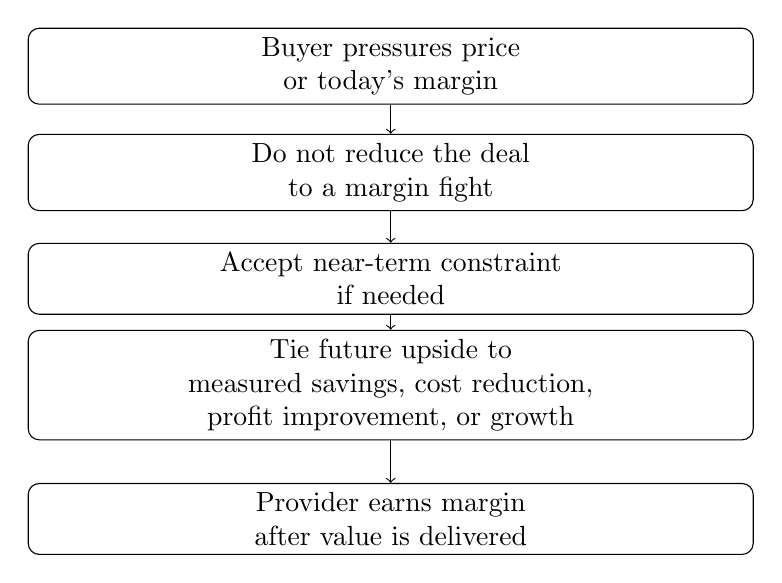
\begin{tikzpicture}[
  node/.style={draw, rounded corners, align=center, text width=0.74\linewidth, minimum height=0.9cm}
]
\node[node] (pressure) at (0,0) {Buyer pressures price\\or today's margin};
\node[node] (choice) at (0,-1.35) {Do not reduce the deal\\to a margin fight};
\node[node] (term) at (0,-2.70) {Accept near-term constraint\\if needed};
\node[node] (measure) at (0,-4.05) {Tie future upside to\\measured savings, cost reduction,\\profit improvement, or growth};
\node[node] (payoff) at (0,-5.75) {Provider earns margin\\after value is delivered};

\draw[->] (pressure) -- (choice);
\draw[->] (choice) -- (term);
\draw[->] (term) -- (measure);
\draw[->] (measure) -- (payoff);
\end{tikzpicture}
\caption{Transcript-derived negotiation pattern. The seller escapes the price-only fight by tying future compensation to measurable customer results.}
\end{figure}

This returns us to the customer-focus section. Louis's sales posture was consultative: if he could not make the customer's business better, there was no deal to earn. His negotiation posture is the same idea written into price: pay more after the business has actually improved.

\section{Summary}

The interview opens with cars, but its serious content is the arithmetic of scale. Delegation turns personal labor into organizational capacity. Retained earnings reduce expensive borrowing. Invoice factoring bridges a dangerous collection gap but extracts a painful cost. Customer contracts create growth only when the company can fund delivery. SOPs, authority, and culture make delegation repeatable. Bankers, peers, and customers become part of the operating system.

The chapter's sequence is:
\[
\text{proof}
\rightarrow
\text{cash-flow discipline}
\rightarrow
\text{stronger balance sheet}
\rightarrow
\text{better capital}
\rightarrow
\text{larger contracts}
\rightarrow
\text{delegated scale}.
\]
The numbers are approximate interview claims, and they should remain source-conscious. But they carry a coherent commercial lesson: wealth here is not presented as one sudden breakthrough. It is a chain of constraints survived in the right order.